\chapter{Progettazione e codifica}

\label{cap:progettazione}

\intro{Durante la fase di progettazione viene definita l'architettura del software, questa operazione consiste nella suddivisione del sistema in componenti distinti, ognuno con compiti differenti.
L'obiettivo è pianificare in maniera chiara tutte le azioni che l'applicativo dovrà svolgere prima di passare effettivamente alla codifica.}

\section{Architettura}
L'architettura (Fig.~\ref{fig:schema-architettura}) pensata prevede l'utilizzo di 4 componenti principali che si occupano di:
\begin{enumerate}
    \item Acquisire gli screenshot.
    \item Effettuare il clustering degli screenshot acquisiti.
    \item Valutare i siti web.
    \item Inviare e-mail promozionali.
\end{enumerate}

\begin{figure}[!h] 
    \centering 
    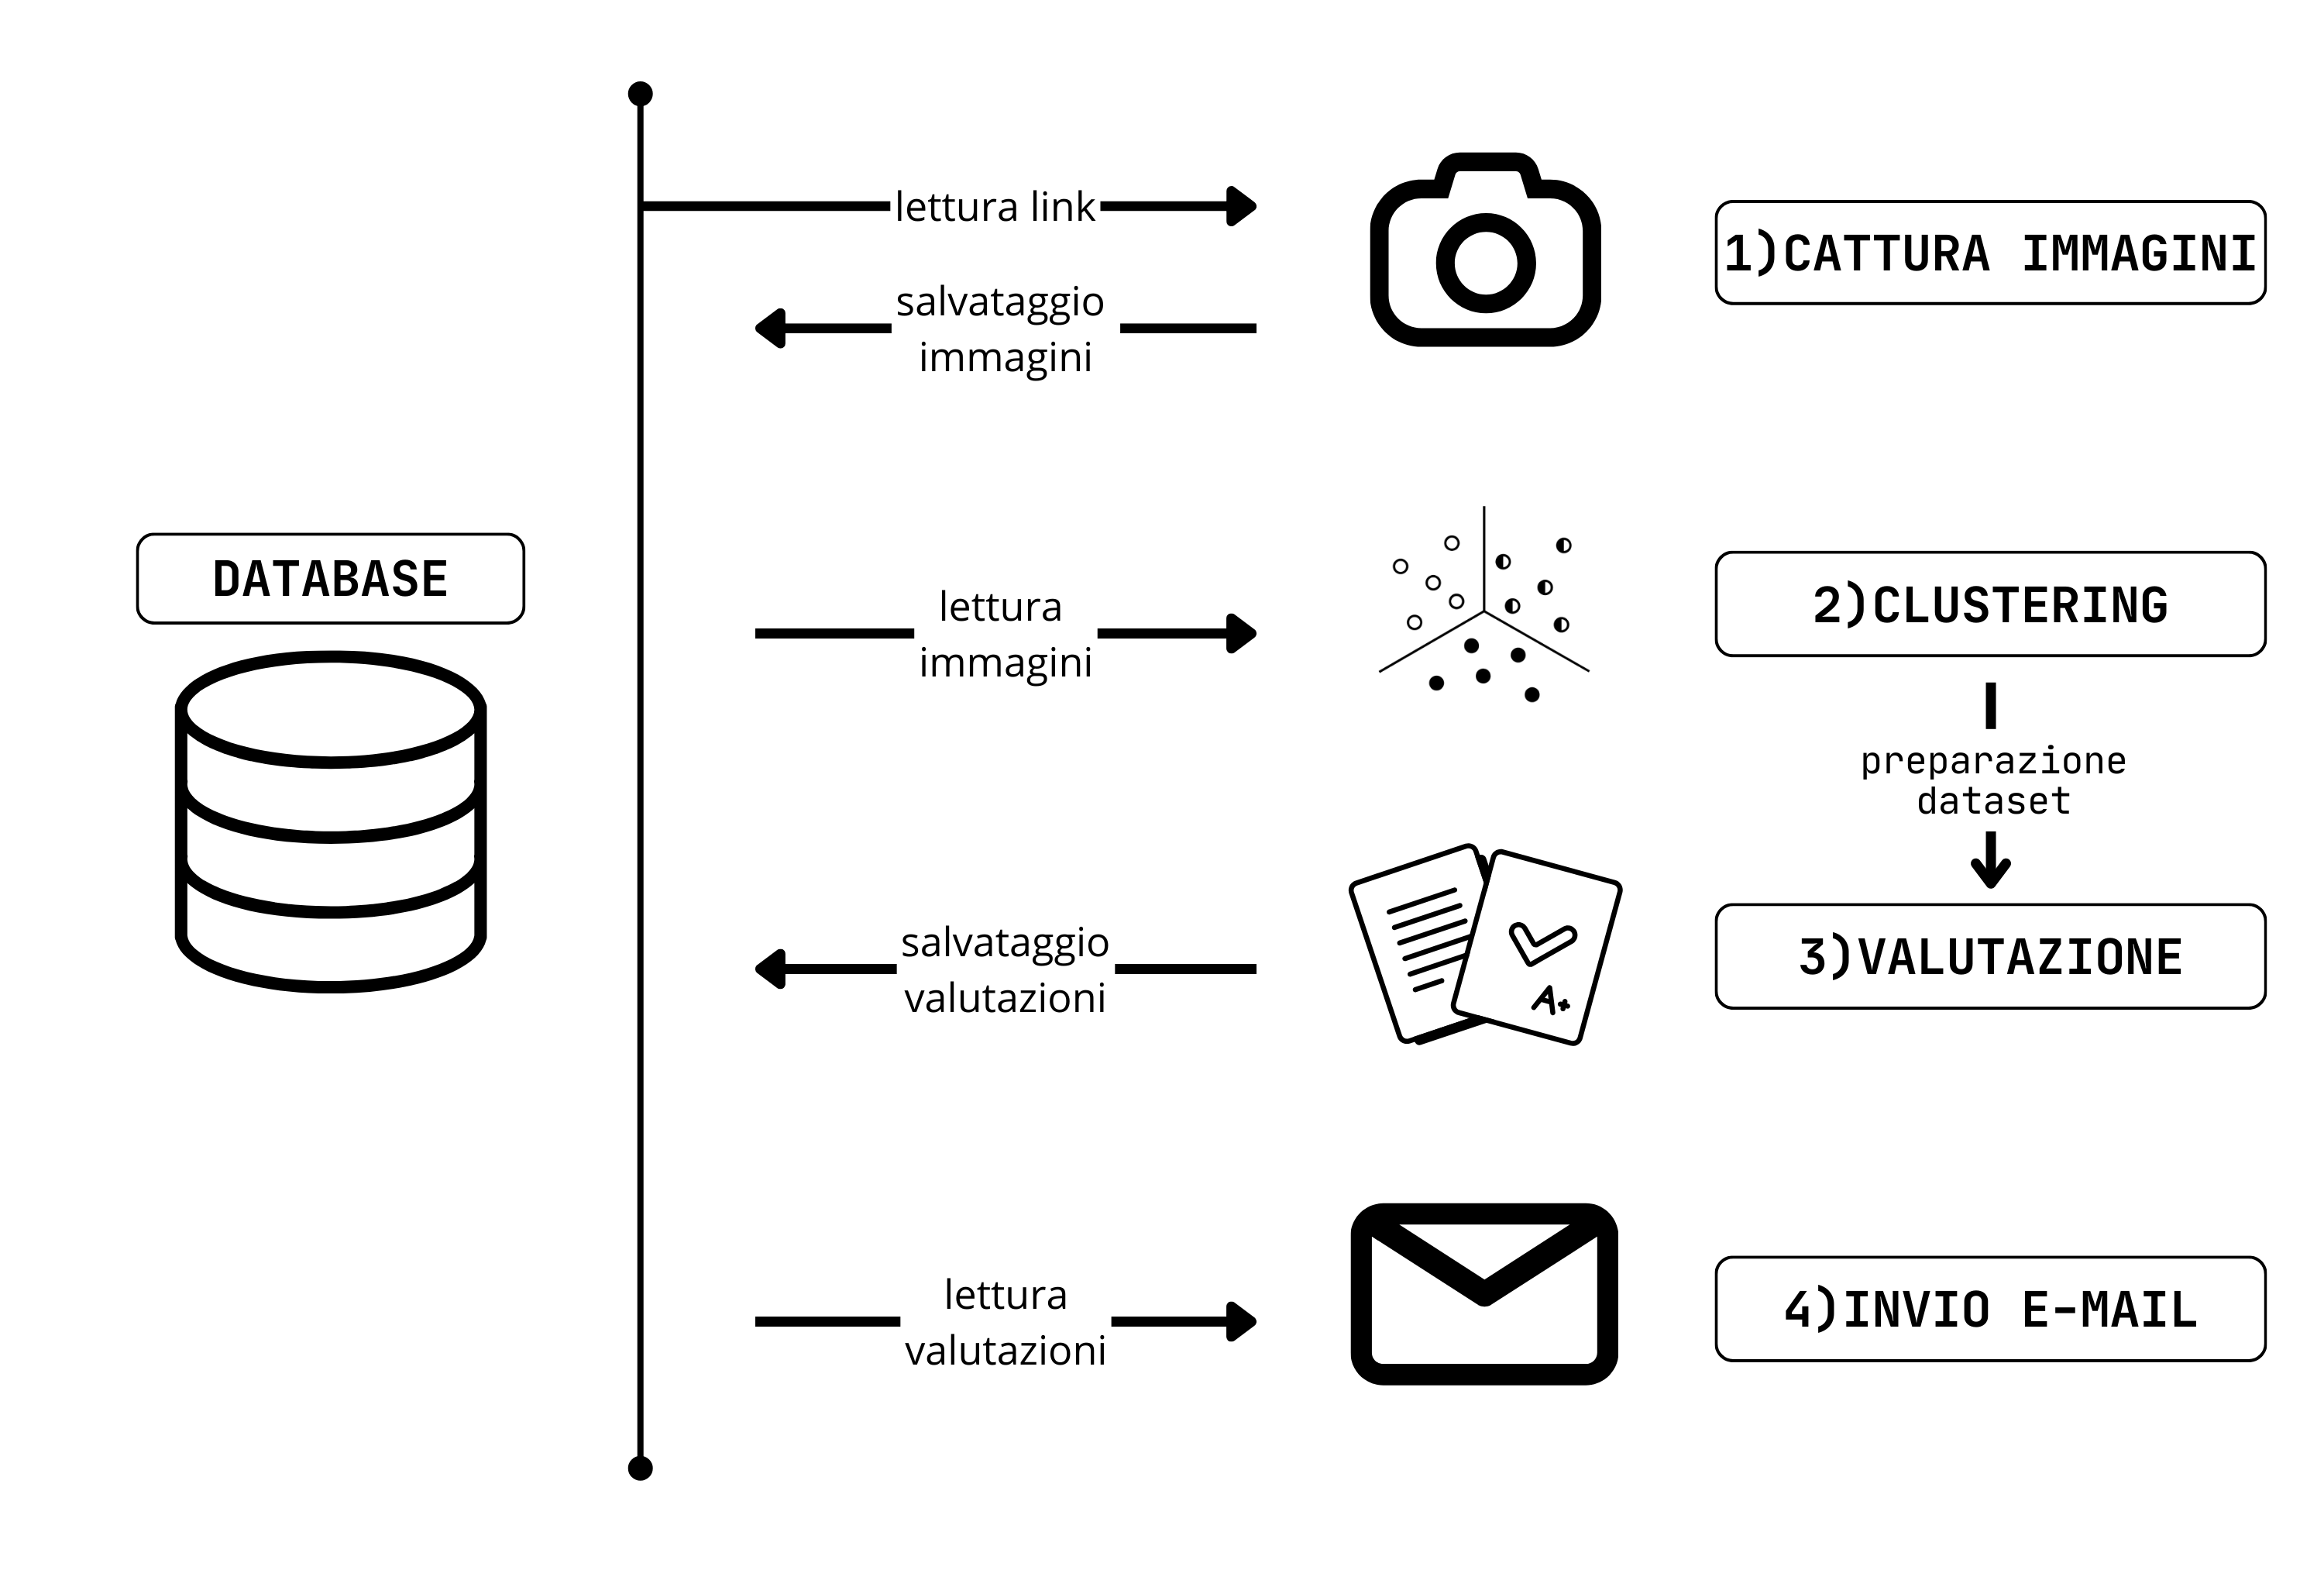
\includegraphics[width=0.9\columnwidth]{progettazione/schema-architettura.png} 
    \caption{Schema architetturale del progetto}
    \label{fig:schema-architettura}
  \end{figure}


\newpage

\section{Cattura immagini}
La prima fase del workflow (Fig.~\ref{fig:schema-cattura}) è composta da uno script Python che usufruisce della libreria Pyppeteer per acquisire gli screenshot dei siti contenuti nel database.
Più precisamente un web-scraper già implementato raccoglie i link delle pagine web dei clienti potenziali, successivamente li carica nel database di SalesCRM, dove verranno infine letti dallo script.
Per funzionare Pyppeteer necessita di chromium, dopo aver effettuato il controllo per verificare se esso sia presente o meno procede con la lettura dei link. 
L'automazione apre ogni indirizzo, aspetta qualche secondo e scatta uno screenshot. 
Tutte le immagini vengono poi convertite in formato Base64 e salvate nel database.

\begin{figure}[!h] 
  \centering 
  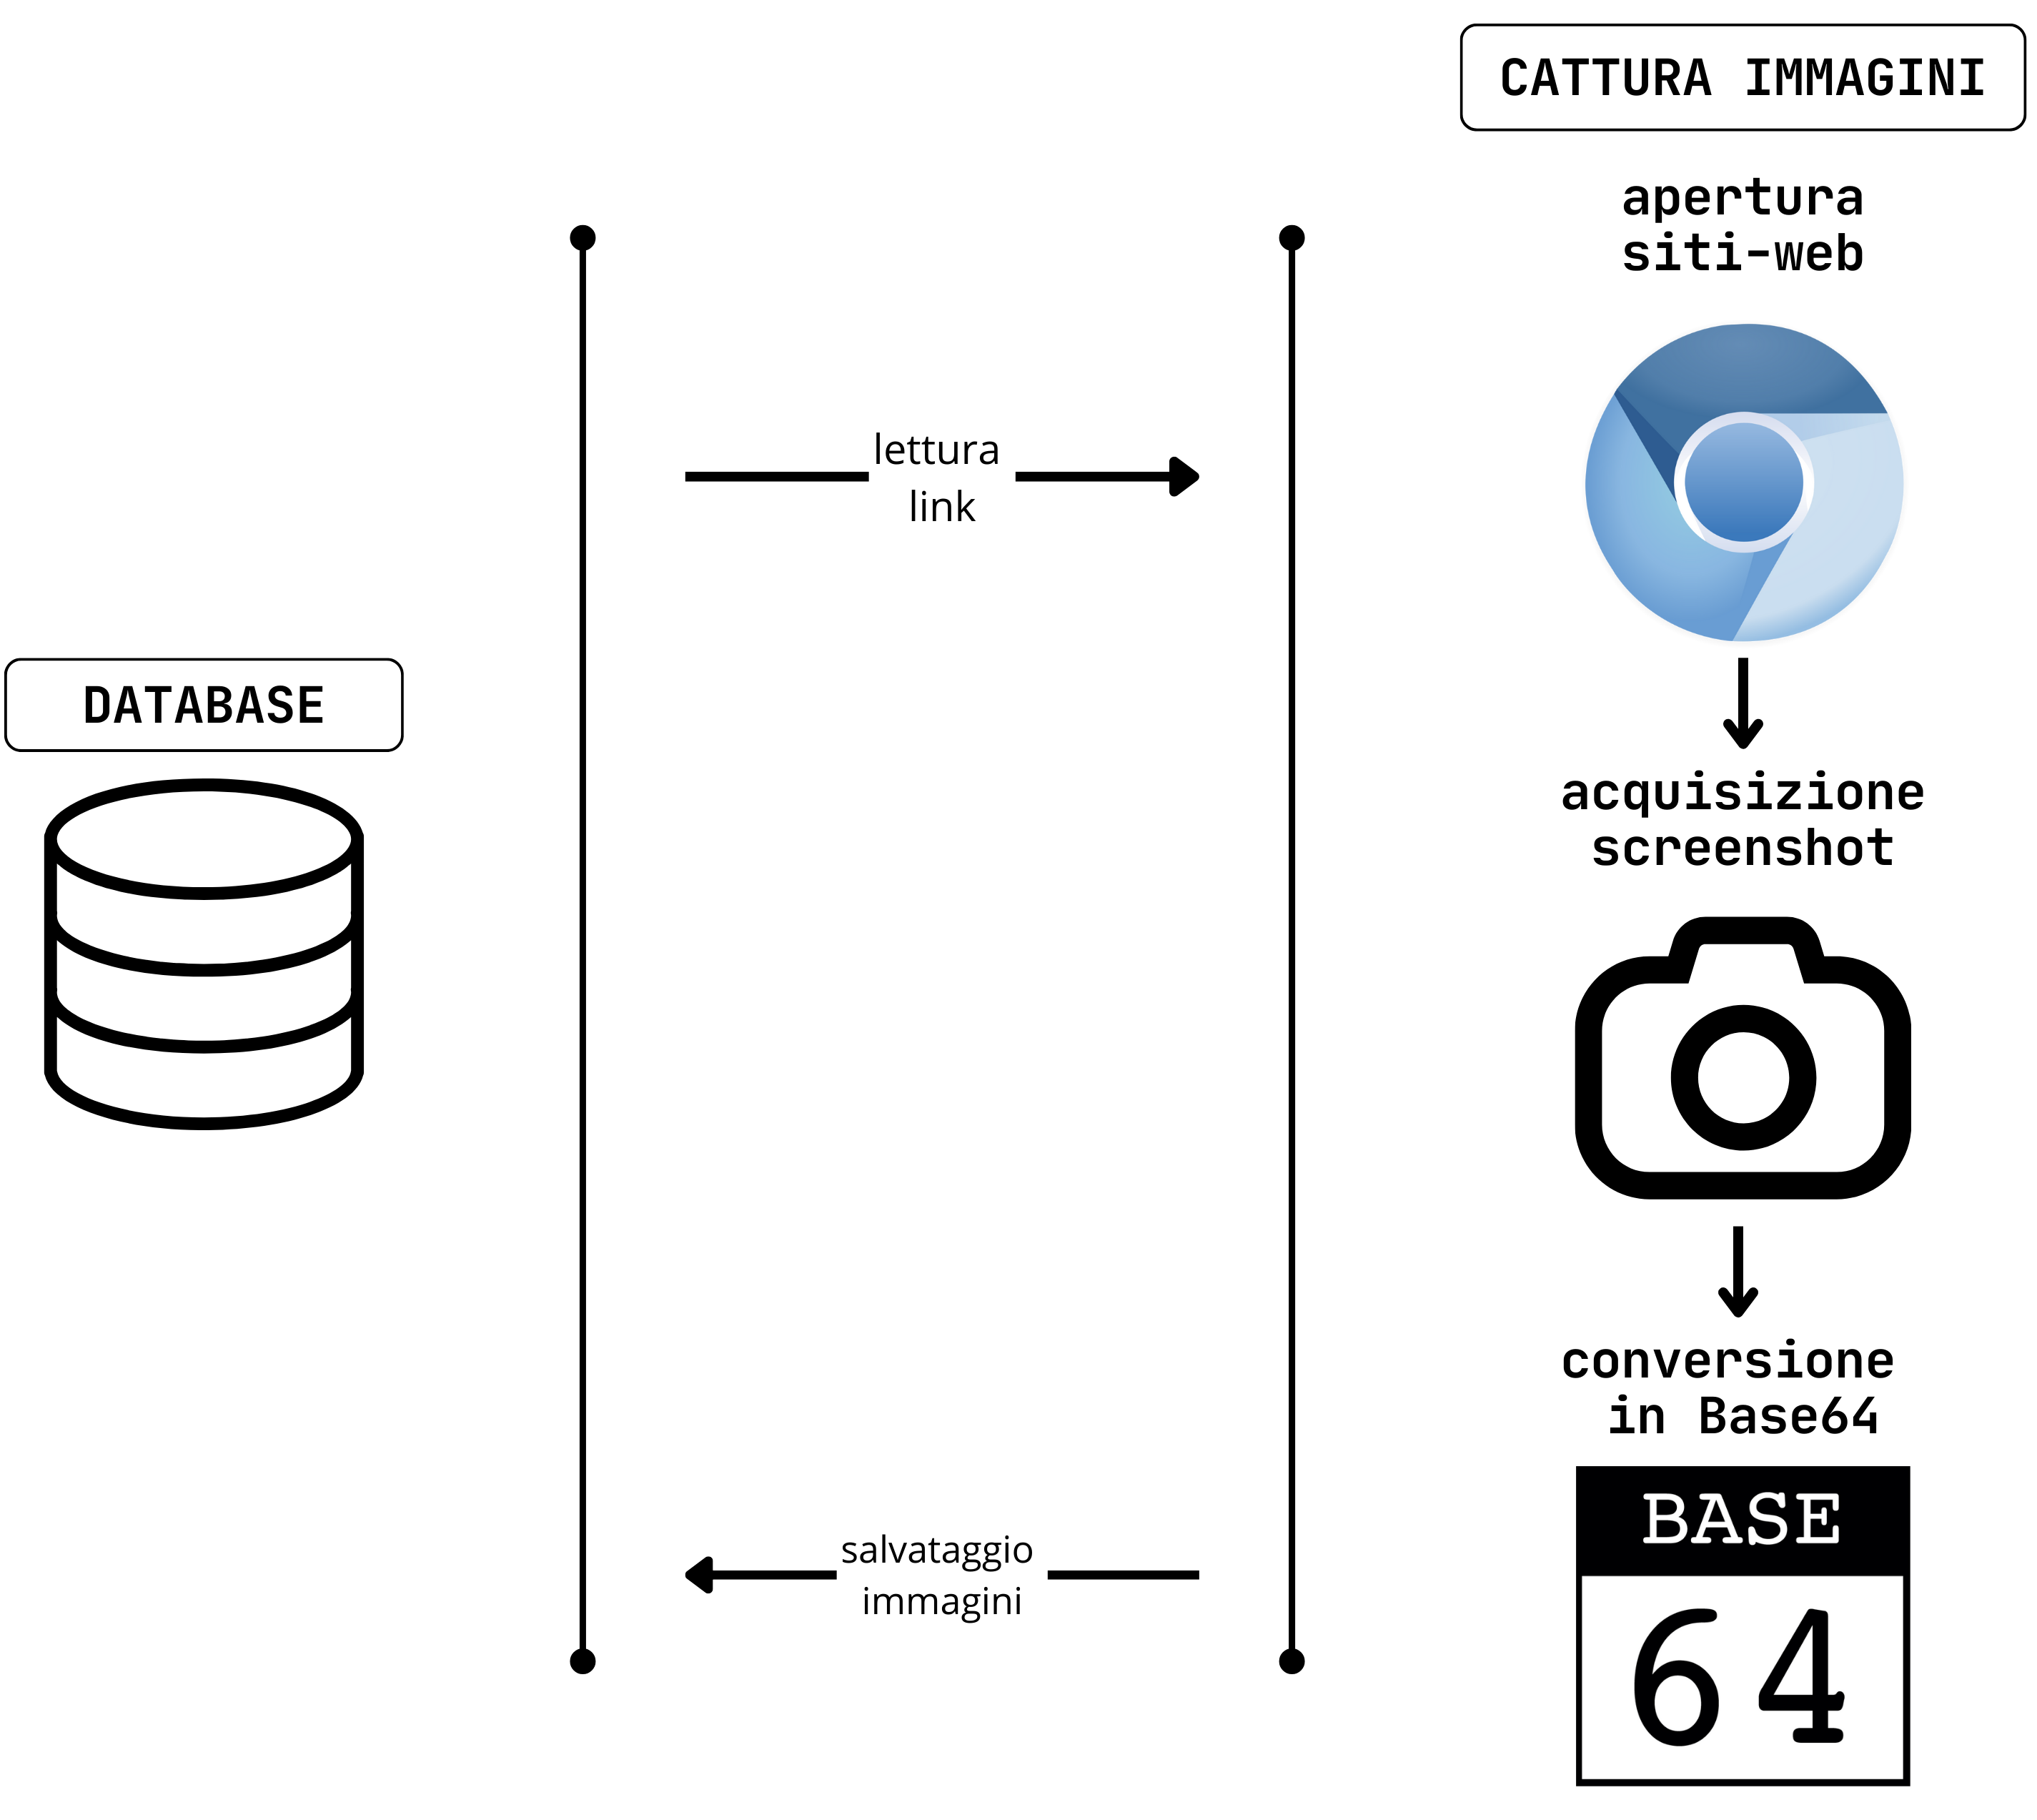
\includegraphics[width=0.5\columnwidth]{progettazione/schema-cattura.png} 
  \caption{Schema della fase di cattura}
  \label{fig:schema-cattura}
\end{figure}

\newpage

\section{Clustering}
\subsection{Preparazione delle immagini}
In seguito alla cattura le immagini vengono lette dal database e convertite in un formato utilizzabile dagli algoritmi di machine learning.
Quindi si passa da un formato Base64 a un formato raster che viene poi nuovamente convertito in un tensore multidimensionale adatto per essere processato.
In questo caso le dimensioni del tensore sono le seguenti (224*224*3):
\begin{itemize}
  \item Altezza dell'immagine
  \item Larghezza dell'immagine 
  \item Numero di canali (Red Green Blue)
\end{itemize} 
Ogni cella viene normalizzata, dividendo il suo contenuto per 255, portando dunque il valore in un intervallo compreso tra 0 e 1.

\subsection{Estrazione delle features}
Per ottenere un dato utilizzabile in modo efficace dall'algoritmo di clustering è necessario modificare ulteriormente le immagini riducendole a un set di features.
Per adempire a questo compito viene utilizzato un CNN Convolutional Neural Network pre-addestrato chiamato ResNet50.
Il modello viene caricato senza i top layers, ossia gli strati densi addetti alla classificazione, per sfruttare esclusivamente la sua abilità di riduzione in features.

\subsection{Applicazione del clustering}
Le features estratte dai layers convoluzionali vengono ridotte a uno stato bidimensionale sfruttando l'analisi dei componenti principali, successivamente viene applicato l'algoritmo dei K-means per l'effettiva suddivisione del dataset in clusters.
Le immagini vengono inserite, in base al cluster a loro assegnato, nelle rispettive cartelle di appartenenza.
Questa operazione viene svolta per semplificare lo step successivo in cui lo sviluppatore deve preparare manualmente il dataset per l'addestramento supervisionato.







%come modello finale è stato scelto resnet 50 poichè più rapido da utilizzare, infatti non necessita di addestramento 

\section{Valutazione}

\section{Invio e-mail}

\section{Database}